% FOR FIGURES, DO NOT USE \psfrag
%
% PLEASE USE THE DRAFT OPTION TO SUBMIT YOUR PAPERS.
\documentclass[draft,jgrga]{agutexSI2019}
%This template serves as both a “table of contents” for the supporting information for your article and as a summary of files.
%
%
%OVERVIEW
%
%Please note that all supporting information will be peer reviewed with your manuscript. It will not be copyedited if the paper is accepted.
%In general, the purpose of the supporting information is to enable authors to provide and archive auxiliary information such as data tables, method information, figures, video, or computer software, in digital formats so that other scientists can use it.
%The key criteria are that the data:
% 1. supplement the main scientific conclusions of the paper but are not essential to the conclusions (with the exception of
%    including %data so the experiment can be reproducible);
% 2. are likely to be usable or used by other scientists working in the field;
% 3. are described with sufficient precision that other scientists can understand them, and
% 4. are not exe files.
%
%USING THIS TEMPLATE
%
%***All references should be included in the reference list of the main paper so that they can be indexed, linked, and counted as citations.  The reference section does not count toward length limits.
%
%All Supporting text and figures should be included in this document. Insert supporting information content into each appropriate section of the template. To add additional captions, simply copy and paste each sample as needed.

%Tables may be included, but can also be uploaded separately, especially if they are larger than 1 page, or if necessary for retaining table formatting. Data sets, large tables, movie files, and audio files should be uploaded separately. Include their captions in this document and list the file name with the caption. You will be prompted to upload these files on the Upload Files tab during the submission process, using file type “Supporting Information (SI)”

%IMPORTANT NOTE ON FIGURES AND TABLES
% Placeholders for figures and tables appear after the \end{article} command, after references.
% DO NOT USE \psfrag or \subfigure commands.
%
 \usepackage{graphicx}
%
%  Uncomment the following command to allow illustrations to print when using Draft:
 \setkeys{Gin}{draft=false}
%
% You may need to use one of these options for graphicx depending on the driver program you are using. 
% [xdvi], [dvipdf], [dvipsone], [dviwindo], [emtex], [dviwin], [pctexps],  [pctexwin],  [pctexhp],  [pctex32], [truetex], [tcidvi], [oztex], [textures]


% Author names in capital letters:
\authorrunninghead{BEGEMAN ET AL.}

% Shorter version of title entered in capital letters:
\titlerunninghead{ICE-SHELF OCEAN BOUNDARY LAYER}

\authoraddr{Corresponding author: C. B. Begeman,
Fluid Dynamics and Solid Mechanics,
Los Alamos National Laboratory,
P.O. Box 1663,
Los Alamos, NM 87545
(cbegeman@lanl.gov)}

\begin{document}

%\includegraphics{agu_pubart-white_reduced.eps}

\title{Supporting Information for ``Ice-shelf ocean boundary layer dynamics from large-eddy simulations"}
%DOI: 10.1002/%insert paper number here%

% List authors by first name or initial followed by last name and
% \thanks{} for author notes.
% Additional author notes should be indicated with \thanks{} (for
% example, for current addresses).
\authors{Carolyn Branecky Begeman\affil{1}, Xylar Asay-Davis\affil{1}, and Luke Van Roekel\affil{1}}
	
\affiliation{1}{Los Alamos National Laboratory, Los Alamos, New Mexico, USA}

\begin{article}

\noindent\textbf{Contents of this file}
%%%Remove or add items as needed%%%
\begin{enumerate}
\item Text S1 to Sx
\item Figures S1 to Sx
\item Tables S1 to Sx
%if Tables are larger than 1 page, upload as separate excel file
\end{enumerate}
\noindent\textbf{Additional Supporting Information (Files uploaded separately)}
\begin{enumerate}
\item Captions for Datasets S1 to Sx
\item Captions for large Tables S1 to Sx (if larger than 1 page, upload as separate excel file)
\item Captions for Movies S1 to Sx
\item Captions for Audio S1 to Sx
\end{enumerate}

\noindent\textbf{Introduction}
%Type or paste your text here. The introduction gives a brief overview of the supporting information. You should include information %about as many of the following as possible (when appropriate):
% 1. a general overview of the kind of data files;
% 2. information about when and how the data were collected or created;
% 3. a general description of processing steps used;
% 4. any known imperfections or anomalies in the data.

%\clearpage

%Delete all unused file types below. Copy/paste for multiples of each file type as needed.
\noindent\textbf{Text S1.}
%Type or paste text here. This should be additional explanatory text, such as: extended descriptions of results, full details of models, extended lists of acknowledgements etc.  It should not be additional discussion, analysis, interpretation or critique. It should not be an additional scientific experiment or paper.
%
%Repeat for any additional Supporting Text

%%Enter Data Set, Movie, and Audio captions here
%%EXAMPLE CAPTIONS

\noindent\textbf{Data Set S1.} %Type or paste caption here.
%upload your dataset(s) to AGU's journal submission site and select "Supporting Information (SI)" as the file type. Following naming %convention: ds01.

%Repeat for any additional Supporting data sets

\noindent\textbf{Movie S1.} %Type or paste caption here.
%upload your movie(s) to AGU's journal submission site and select, "Supporting Information %(SI)" as the file type. Following naming convention: ms01.

%Repeat any additional Supporting movies

%%% End of body of article:
%%%%%%%%%%%%%%%%%%%%%%%%%%%%%%%%%%%%%%%%%%%%%%%%%%%%%%%%%%%%%%%%
%
% Optional Notation section goes here
%
% Notation -- End each entry with a period.
% \begin{notation}
% Term & definition.\\
% Second term & second definition.\\
% \end{notation}
%%%%%%%%%%%%%%%%%%%%%%%%%%%%%%%%%%%%%%%%%%%%%%%%%%%%%%%%%%%%%%%%


\bibliography{references}
% no need to specify bibliographystyle
%
% Note that ALL references in this supporting information file must also be referenced in the primary manuscript
% if you get an error about newblock being undefined, uncomment this line:
%\newcommand{\newblock}{}
%\bibliography{<name of your .bib file>} 

% \end{article} must follow the references section, before the figures and tables.
\end{article}
\clearpage

% Copy/paste for multiples of each file type as needed.

% enter figures and tables below here: %%%%%%%
\begin{figure}[]
    \setfigurenum{S1}
    \centering
    \begin{minipage}{0.5\textwidth}
        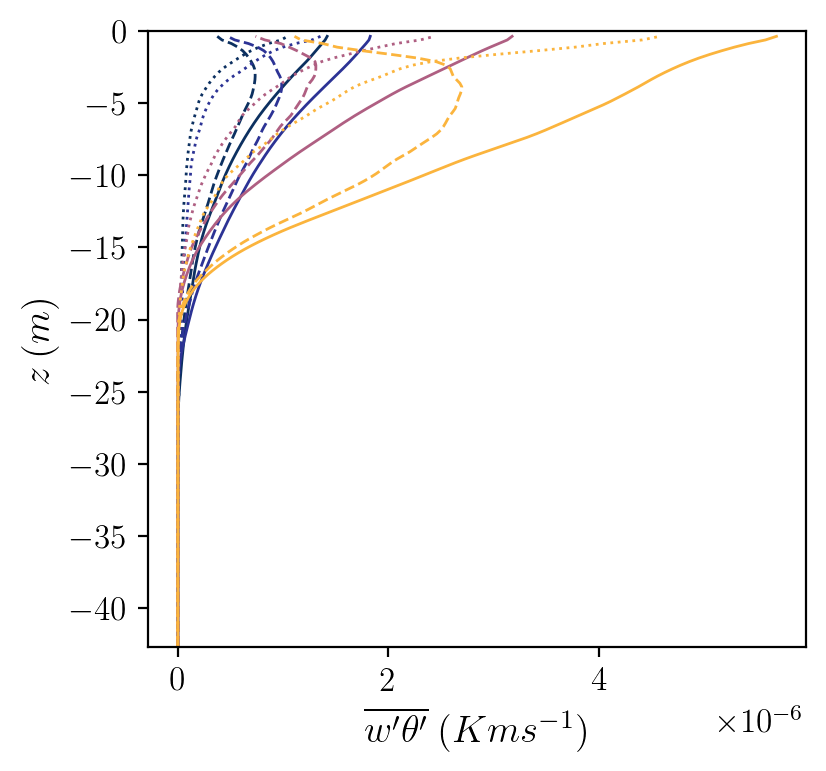
\includegraphics[trim={0 0 0 0},clip, width=\textwidth]{Figures/heatflux_res_sgs_cmp_dT_8h_tav13h_z_profile.png}
    \end{minipage}%
    \begin{minipage}{0.5\textwidth}
        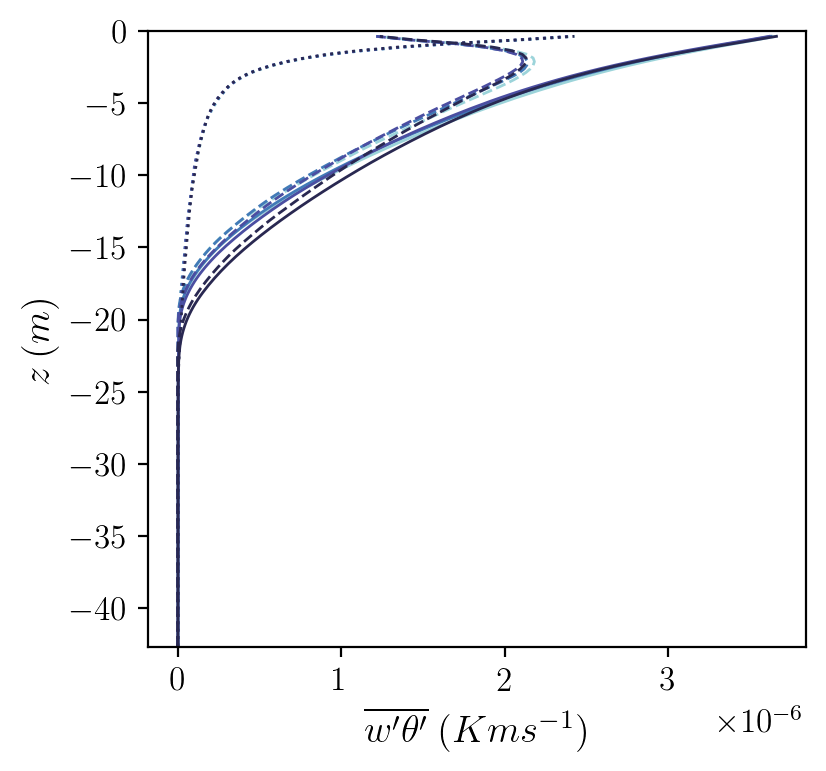
\includegraphics[trim={0 0 0 0},clip, width=\textwidth]{Figures/heatflux_res_sgs_cmp_dslope_8h_tav13h_z_profile.png}
    \end{minipage}
    \begin{minipage}{0.5\textwidth}
        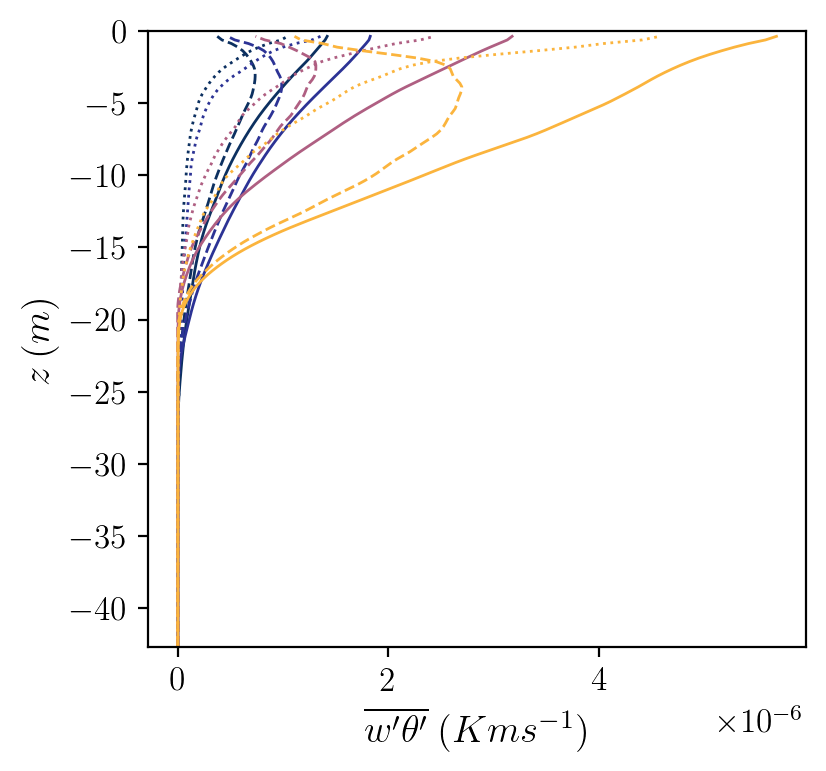
\includegraphics[trim={0 0 0 0},clip, width=\textwidth]{Figures/heatflux_res_sgs_cmp_dT_43h_tav13h_z_profile.png}
    \end{minipage}%
    \begin{minipage}{0.5\textwidth}
        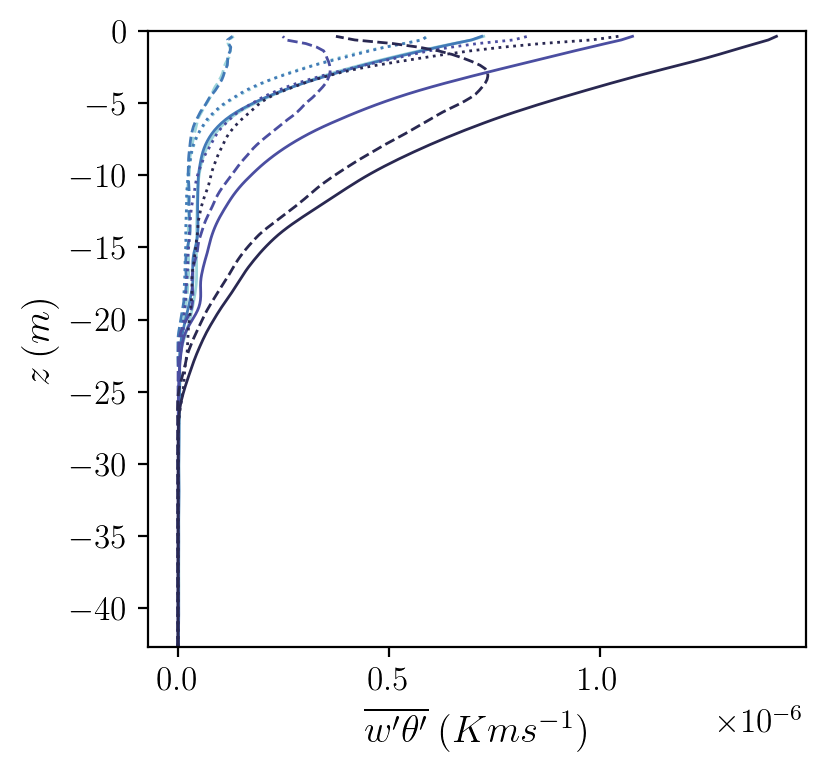
\includegraphics[trim={0 0 0 0},clip, width=\textwidth]{Figures/heatflux_res_sgs_cmp_dslope_43h_tav13h_z_profile.png}
    \end{minipage}
    \caption{Vertical heat flux depth-profiles averaged over one inertial period for (a,c) thermal driving simulations and (b,d) variable slope simulations. Profiles shown in (a,b) are averaged over the first inertial period after a 2h spin-up, (b,d) over the last inertial period. Solid lines represent the total flux, dashed resolved flux and dotted subgrid flux. Colors correspond to those shown in Figure 1.}
    \label{fig:res_sgs_flux}
\end{figure}

\begin{figure}[]
    \setfigurenum{S2}
    \centering
    \begin{minipage}{0.5\textwidth}
        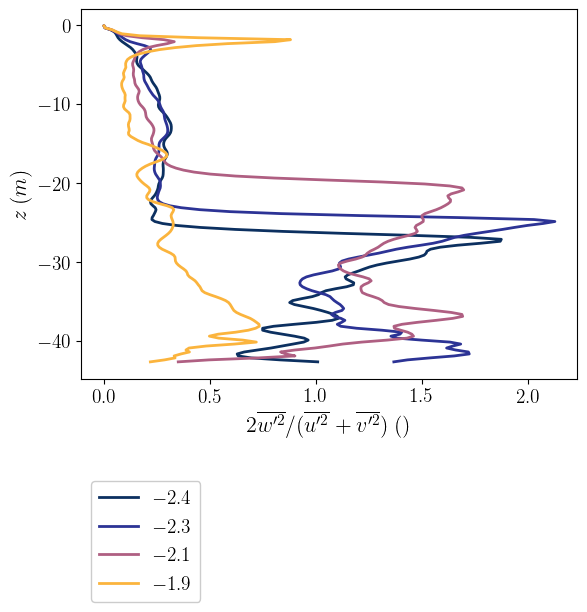
\includegraphics[trim={0 4cm 0 0},clip,width=\textwidth]{Figures/vel_var_ratio_cmp_dT_40hr_tav1_z_profile.png}
    \end{minipage}%
    \begin{minipage}{0.5\textwidth}
        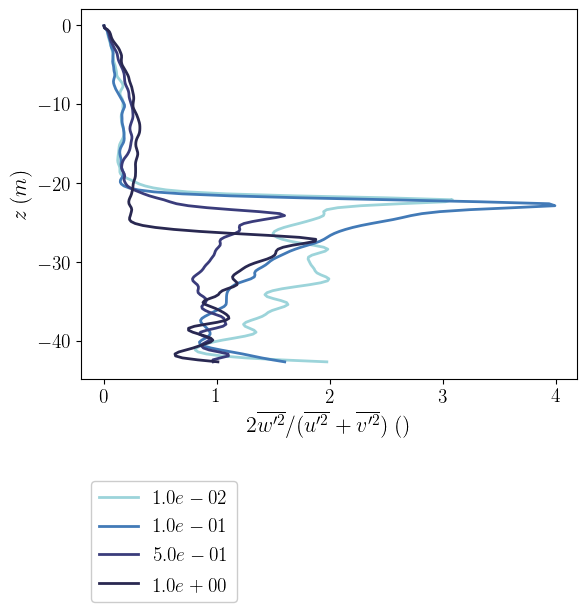
\includegraphics[trim={0 4cm 0 0},clip,width=\textwidth]{Figures/vel_var_ratio_cmp_dslope_40hr_tav1_z_profile.png}
    \end{minipage}
    \caption{Ratio of vertical to horizontal velocity variance for (a) thermal driving simulations and (b) variable slope simulations at 40h.}
    \label{fig:vel_var_ratio}
\end{figure}

\begin{figure}
    \setfigurenum{S3}
    \centering
    \begin{minipage}{0.5\textwidth}
        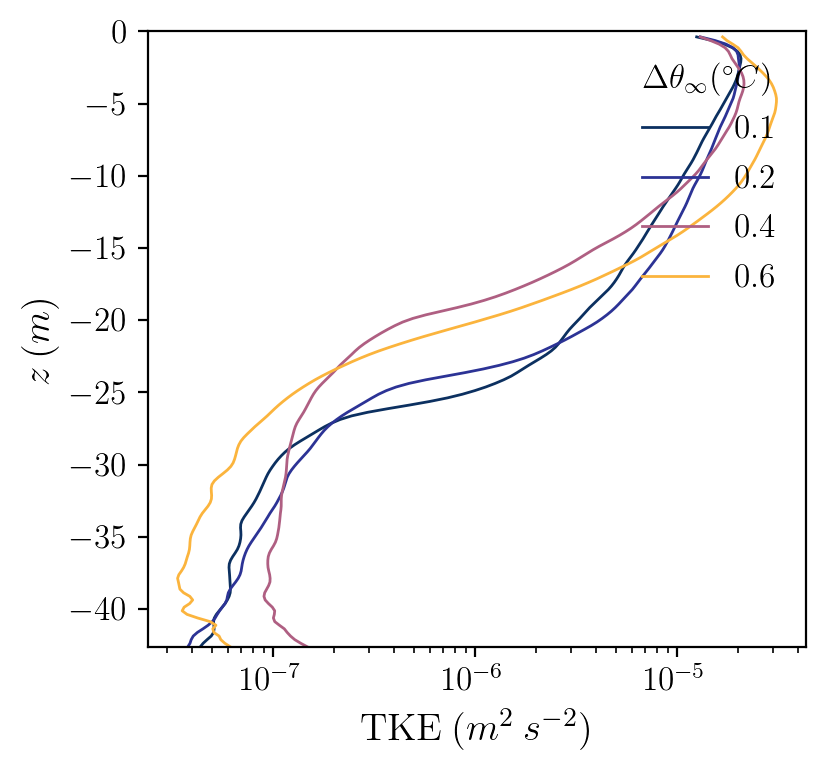
\includegraphics[trim={0 0 0 0},clip, width=\textwidth]{Figures/eres_cmp_dT_43h_tav13h_z_profile.png}
    \end{minipage}%
    \begin{minipage}{0.5\textwidth}
        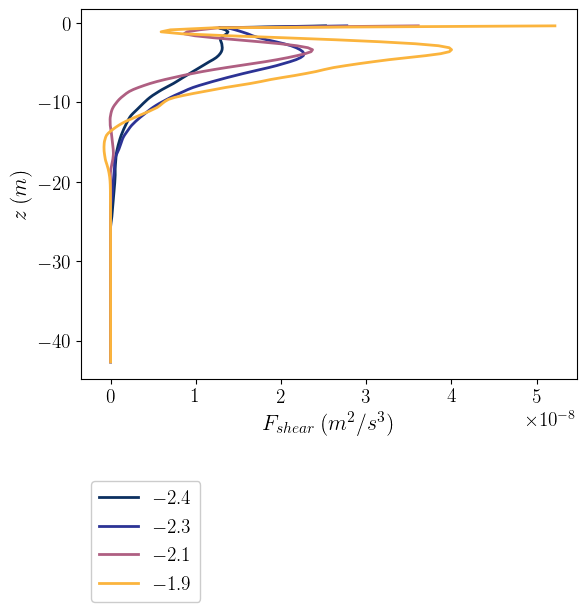
\includegraphics[trim={0 0 0 0},clip,width=\textwidth]{Figures/Fshear_cmp_dT_43h_tav13h_z_profile.png}    
    \end{minipage}
    \newline
    \begin{minipage}{0.5\textwidth}
        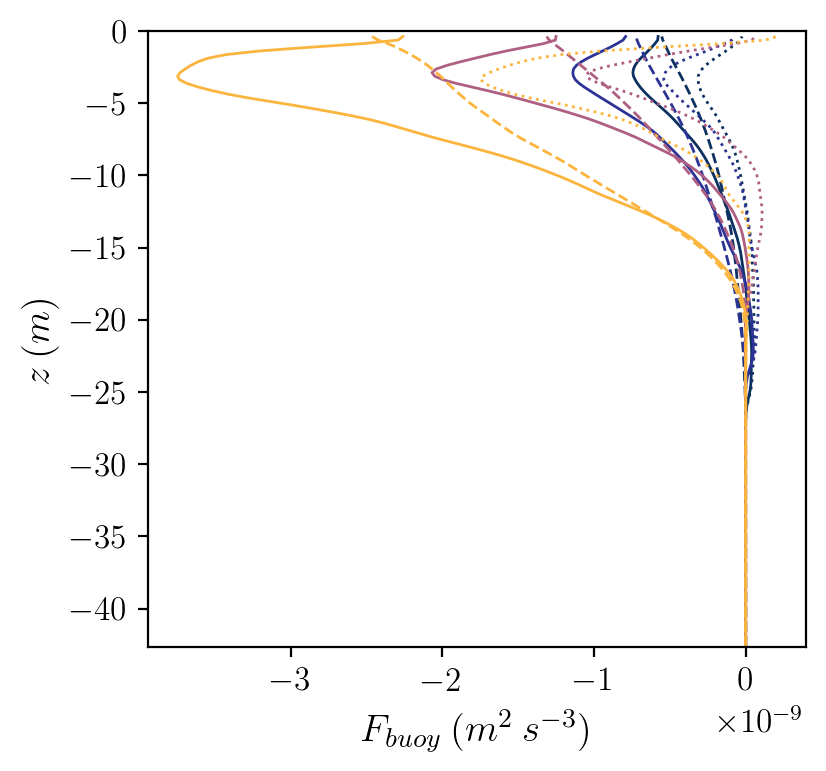
\includegraphics[trim={0 0 0 0},clip,width=\textwidth]{Figures/Fbuoy_cmp_dT_43h_tav13h_z_profile.png}
    \end{minipage}%
    \begin{minipage}{0.5\textwidth}
        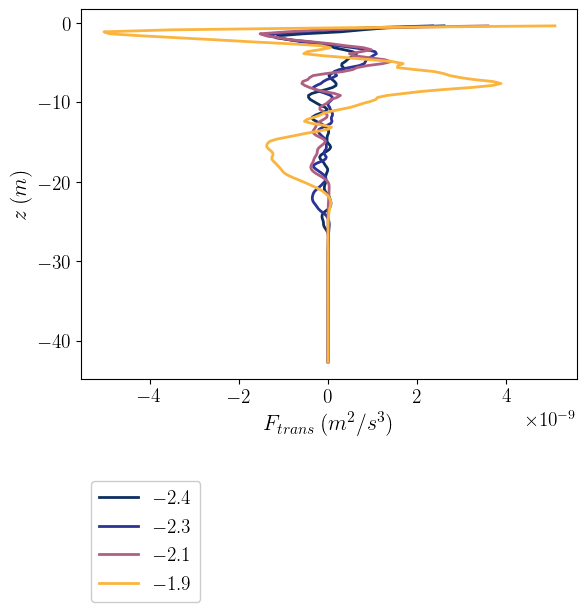
\includegraphics[trim={0 0 0 0},clip,width=\textwidth]{Figures/Ftrans_cmp_dT_43h_tav13h_z_profile.png}
    \end{minipage}
    \caption{(a) Simulated turbulent kinetic energy for variable thermal driving simulations averaged over the last inertial period and (b-d) turbulent kinetic energy production terms over the same period. (b) Shear production. (c) Buoyancy production. The total buoyancy production is shown with solid lines, vertical component dashed, and upslope component dotted. (d) TKE transport. Positive denotes production, negative destruction. Note that the x-axis scales differ between panels.}
    \label{fig:tke_budget}
    % Change x-axis label for buoyancy production terms
\end{figure}

\begin{figure}[]
    \setfigurenum{S4}
    \centering
    \begin{minipage}{0.5\textwidth}
        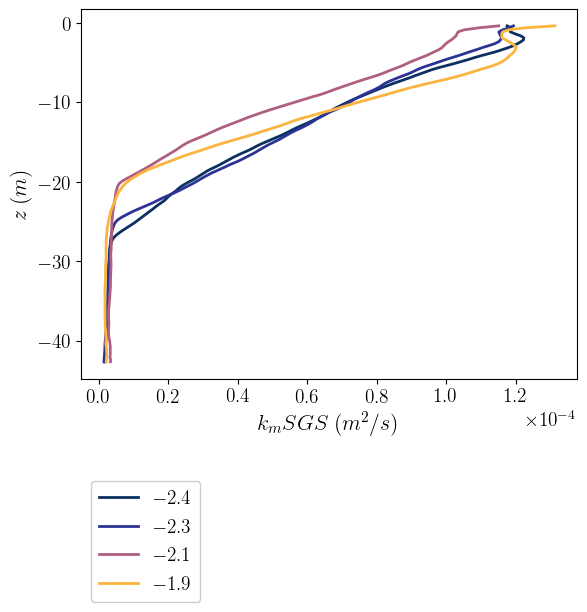
\includegraphics[trim={0 4.5cm 0 0},clip, width=\textwidth]{Figures/km_cmp_dT_44h_tav12_z_profile.png}
    \end{minipage}%
    \begin{minipage}{0.5\textwidth}
        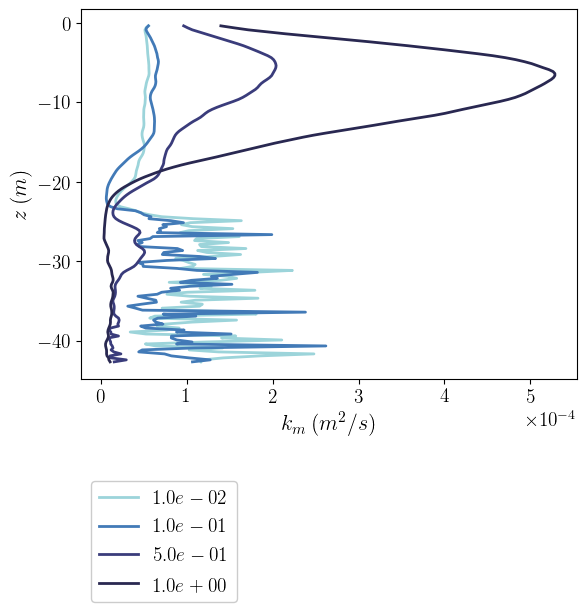
\includegraphics[trim={0 4.5cm 0 0},clip, width=\textwidth]{Figures/km_cmp_slope_46h_tav12_z_profile.png}
    \end{minipage}
    \caption{Effective vertical diffusivity for momentum flux from (a) thermal driving simulations and (b) slope-varying simulations over the last inertial period. Fluctuations below the boundary layer ($\sim$20 m) are not interpretable due to low velocity gradients. }
    \label{fig:km}
\end{figure}

\begin{figure}[]
    \setfigurenum{S5}
    \centering
    \begin{minipage}{0.5\textwidth}
        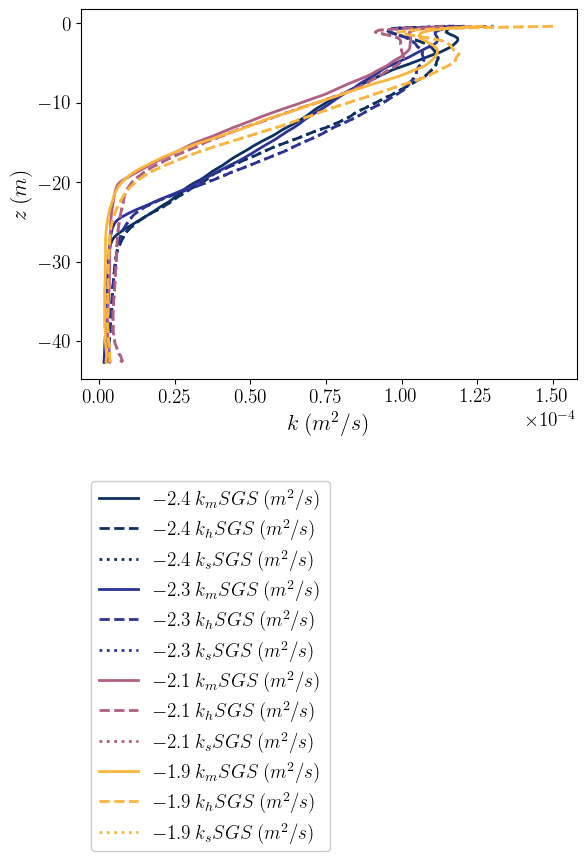
\includegraphics[trim={0 0 0 0},clip, width=\textwidth]{Figures/k_cmp_dT_43h_tav13h_z_profile.png}
    \end{minipage}%
    \begin{minipage}{0.5\textwidth}
        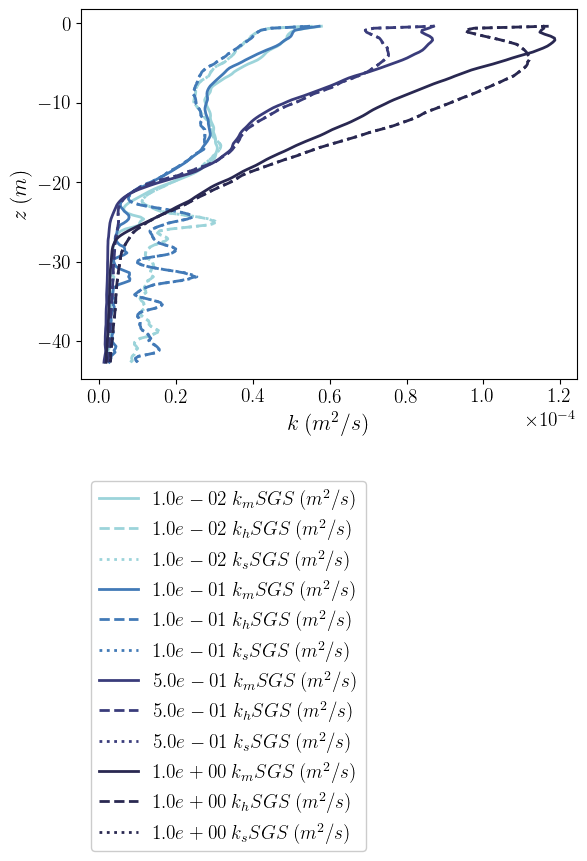
\includegraphics[trim={0 0 0 0},clip, width=\textwidth]{Figures/k_cmp_dslope_43h_tav13h_z_profile.png}
    \end{minipage}
    \caption{Sub-grid vertical diffusivity for momentum flux for momentum (solid), heat (dashed) and salt (dotted) for (a) thermal driving simulations and (b) variable slope simulations. Heat and salt diffusivities curves are visually indistinguishable.}
    \label{fig:k_all}
    %TODO replace legend
\end{figure}

\begin{figure}[]
    \setfigurenum{S6}
    \centering
    \begin{minipage}{0.5\textwidth}
        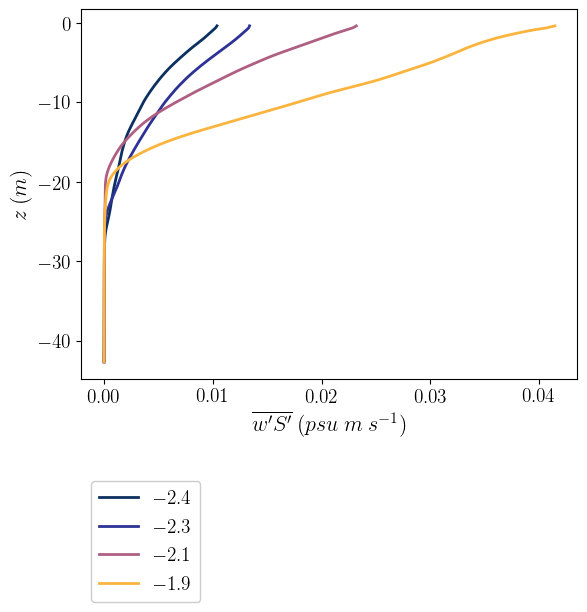
\includegraphics[trim={0 4cm 0 0},clip, width=\textwidth]{Figures/wsa_cmp_dT_43h_tav13_z_profile.png}
    \end{minipage}%
    \begin{minipage}{0.5\textwidth}
        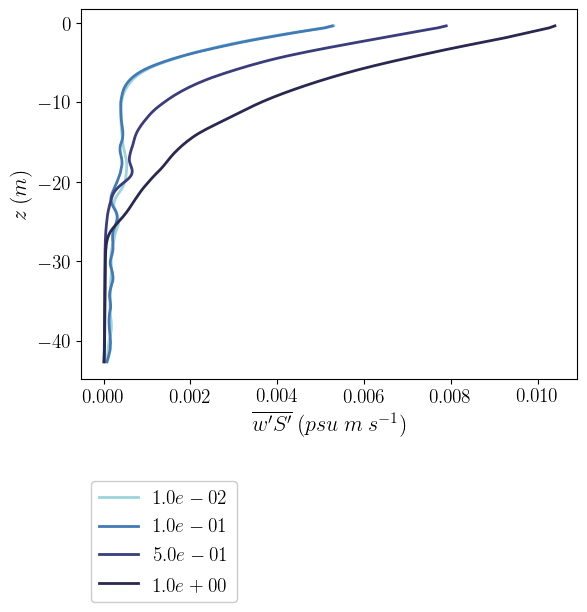
\includegraphics[trim={0 4cm 0 0},clip, width=\textwidth]{Figures/wsa_cmp_dslope_43h_tav13_z_profile.png}
    \end{minipage}
    \caption{Total vertical salt flux depth-profiles averaged over one inertial period for (a) thermal driving simulations and (b) variable slope simulations.}
    \label{fig:saltflux}
    %TODO replace legend
\end{figure}%

\begin{figure}
    \setfigurenum{S7}
    \centering
    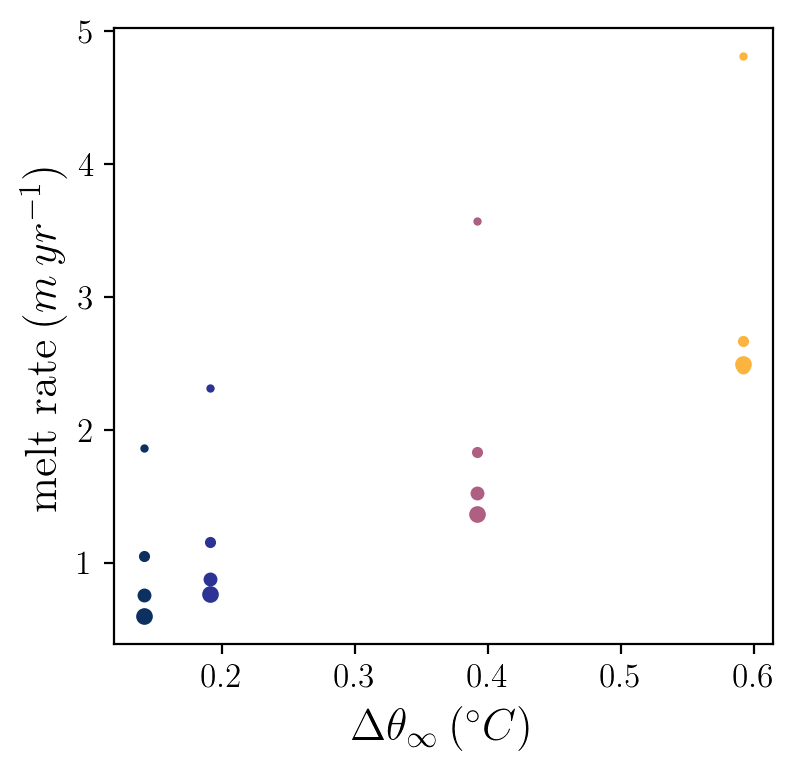
\includegraphics{Figures/melt_dT_cmp_dT_43h_tav13h_cycles.png}
    \caption{Relationship between far-field thermal driving and melt rate. Same as Figure 7a but with values averaged over each inertial cycle. The largest points correspond to the fourth and last inertial cycle with progressively smaller points for previous inertial cycles. }
    \label{fig:melt_sensitivity_cycles}
\end{figure}%
%
%
% EXAMPLE FIGURES
% ---------------
% If you get an error about an unknown bounding box, try specifying the width and height of the figure with the natwidth and natheight options.
% \begin{figure}
%\setfigurenum{S1} %%You can change number for each figure if you want, not required. "S" prepended automatically.
% \noindent\includegraphics[natwidth=800px,natheight=600px]{samplefigure.eps}
%\caption{caption}
%\label{epsfiguresample}
%\end{figure}
%
%
% Giving latex a width will help it to scale the figure properly. A simple trick is to use \textwidth. Try this if large figures run off the side of the page.
% \begin{figure}
% \noindent\includegraphics[width=\textwidth]{anothersample.png}
%\caption{caption}
%\label{pngfiguresample}
%\end{figure}
%
%
%\begin{figure}
%\noindent\includegraphics[width=\textwidth]{athirdsample.pdf}
%\caption{A pdf test figure}
%\label{pdffiguresample}
%\end{figure}
%
% PDFLatex does not seem to be able to process EPS figures. You may want to try the epstopdf package.
%
%
% ---------------
% EXAMPLE TABLE
%
%\begin{table}
%\settablenum{S1} %%Change number for each table
%\caption{Time of the Transition Between Phase 1 and Phase 2\tablenotemark{a}}
%\centering
%\begin{tabular}{l c}
%\hline
% Run  & Time (min)  \\
%\hline
%  $l1$  & 260   \\
%  $l2$  & 300   \\
%  $l3$  & 340   \\
%  $h1$  & 270   \\
%  $h2$  & 250   \\
%  $h3$  & 380   \\
%  $r1$  & 370   \\
%  $r2$  & 390   \\
%\hline
%\end{tabular}
%\tablenotetext{a}{Footnote text here.}
%\end{table}
% ---------------
%
% EXAMPLE LARGE TABLE (UPLOADED SEPARATELY)
%\begin{table}
%\settablenum{S1} %%Change number for each table
%\caption{Time of the Transition Between Phase 1 and Phase 2\tablenotemark{a}}
%\end{table}


\end{document}

%%%%%%%%%%%%%%%%%%%%%%%%%%%%%%%%%%%%%%%%%%%%%%%%%%%%%%%%%%%%%%%

% More Information and Advice:

%% ------------------------------------------------------------------------ %%
%
%  SECTION HEADS
%
%% ------------------------------------------------------------------------ %%

% Capitalize the first letter of each word (except for
% prepositions, conjunctions, and articles that are
% three or fewer letters).

% AGU follows standard outline style; therefore, there cannot be a section 1 without
% a section 2, or a section 2.3.1 without a section 2.3.2.
% Please make sure your section numbers are balanced.
% ---------------
% Level 1 head
%
% Use the \section{} command to identify level 1 heads;
% type the appropriate head wording between the curly
% brackets, as shown below.
%
%An example:
%\section{Level 1 Head: Introduction}
%
% ---------------
% Level 2 head
%
% Use the \subsection{} command to identify level 2 heads.
%An example:
%\subsection{Level 2 Head}
%
% ---------------
% Level 3 head
%
% Use the \subsubsection{} command to identify level 3 heads
%An example:
%\subsubsection{Level 3 Head}
%
%---------------
% Level 4 head
%
% Use the \subsubsubsection{} command to identify level 3 heads
% An example:
%\subsubsubsection{Level 4 Head} An example.
%
%% ------------------------------------------------------------------------ %%
%
%  IN-TEXT LISTS
%
%% ------------------------------------------------------------------------ %%
%
% Do not use bulleted lists; enumerated lists are okay.
% \begin{enumerate}
% \item
% \item
% \item
% \end{enumerate}
%
%% ------------------------------------------------------------------------ %%
%
%  EQUATIONS
%
%% ------------------------------------------------------------------------ %%

% Single-line equations are centered.
% Equation arrays will appear left-aligned.

% Math coded inside display math mode \[ ...\]
%  will not be numbered, e.g.,:
%  \[ x^2=y^2 + z^2\]

%  Math coded inside \begin{equation} and \end{equation} will
%  be automatically numbered, e.g.,:
%  \begin{equation}
%  x^2=y^2 + z^2
%  \end{equation}

% IF YOU HAVE MULTI-LINE EQUATIONS, PLEASE
% BREAK THE EQUATIONS INTO TWO OR MORE LINES
% OF SINGLE COLUMN WIDTH (20 pc, 8.3 cm)
% using double backslashes (\\).

% To create multiline equations, use the
% \begin{eqnarray} and \end{eqnarray} environment
% as demonstrated below.
% \begin{eqnarray}
%   x_{1} & = & (x - x_{0}) \cos \Theta \nonumber \\
%         && + (y - y_{0}) \sin \Theta  \nonumber \\
%   y_{1} & = & -(x - x_{0}) \sin \Theta \nonumber \\
%         && + (y - y_{0}) \cos \Theta.
% \end{eqnarray}

%If you don't want an equation number, use the star form:
%\begin{eqnarray*}...\end{eqnarray*}

% Break each line at a sign of operation
% (+, -, etc.) if possible, with the sign of operation
% on the new line.

% Indent second and subsequent lines to align with
% the first character following the equal sign on the
% first line.

% Use an \hspace{} command to insert horizontal space
% into your equation if necessary. Place an appropriate
% unit of measure between the curly braces, e.g.
% \hspace{1in}; you may have to experiment to achieve
% the correct amount of space.


%% ------------------------------------------------------------------------ %%
%
%  EQUATION NUMBERING: COUNTER
%
%% ------------------------------------------------------------------------ %%

% You may change equation numbering by resetting
% the equation counter or by explicitly numbering
% an equation.

% To explicitly number an equation, type \eqnum{}
% (with the desired number between the brackets)
% after the \begin{equation} or \begin{eqnarray}
% command.  The \eqnum{} command will affect only
% the equation it appears with; LaTeX will number
% any equations appearing later in the manuscript
% according to the equation counter.
%

% If you have a multiline equation that needs only
% one equation number, use a \nonumber command in
% front of the double backslashes (\\) as shown in
% the multiline equation above.

%% ------------------------------------------------------------------------ %%
%
%  SIDEWAYS FIGURE AND TABLE EXAMPLES
%
%% ------------------------------------------------------------------------ %%
%
% For tables and figures, add \usepackage{rotating} to the paper and add the rotating.sty file to the folder.
% AGU prefers the use of {sidewaystable} over {landscapetable} as it causes fewer problems.
%
% \begin{sidewaysfigure}
% \includegraphics[width=20pc]{samplefigure.eps}
% \caption{caption here}
% \label{label_here}
% \end{sidewaysfigure}
%
%
%
% \begin{sidewaystable}
% \caption{}
% \begin{tabular}
% Table layout here.
% \end{tabular}
% \end{sidewaystable}
%
%
